\documentclass[12pt]{article}
\usepackage{titlesec}
\usepackage{float}
\usepackage{graphicx}

\usepackage{hyperref}
\hypersetup{
    colorlinks,
    citecolor=black,
    filecolor=black,
    linkcolor=black,
    urlcolor=black
}

\begin{document}

\title{Design Document} 
\author{Team: The Outsiders\\ \\ Kirk Montour (montour)\\ Syed Gardezi (gardezsh)}
\date{\today}
  
\maketitle

\pagebreak

\tableofcontents

\pagebreak

\listoffigures

\section{User Interface Elements Description}
In this part of the document, we will provide the the description of the user interface (UI) design of our Content Management System (CMS).

\subsection{Acronyms}

\begin{table}[h]
\centering
\caption{Acronyms used}
\label{my-label}
\begin{tabular}{|l|l|}
\hline
UI  & User Interface            \\ \hline
CMS & Content Management System \\ \hline
\end{tabular}
\end{table}


\subsection{Navigation Flow}
The following tasks lay out the navigation flow of the CMS with all possible navigation option at each task execution.

\begin{enumerate}
  \item When a users enters the URL of the administration site into the browser, they will be brought to the landing page of our CMS, this landing page is the Administration site login page.
  \item Once the user is on the Administration site login page, they can choose to login to the the CMS.
  \item Users after logging in have the ability to create new basic user accounts.
  \item Users will also have the ability to edit their accounts by clicking on the ''Users'' menu in the navigation bar which will bring them to the User Management page.
  \item Similar to the edit user option, users will have the ability to delete their accounts once they're logged in. For this, they will use the ''Users'' menu to navigate to the User Management page.
  \item After logging in, users will be brought to the Page Management page where they will be able to add new pages or edit existing pages.
  \item Logged in users can also change the theme for their site by using ''Themes'' menu in the navigation bar.
\end{enumerate} 


\begin{figure}[H]
  
  \centering
    \includegraphics[width=\textwidth,height=\textheight,keepaspectratio]{pics/NavigationFlow.png}
    \caption{Navigation flow of Content Management System}
\end{figure}


\subsection{Donald Norman’'s Design Principles}
We will be using Donald Norman's design principles to guide us in our User Interface (UI) design for our Content Management System (CMS). These principles include: 

\begin{enumerate}
  \item \textbf{Visibility:} The more visible functions are, the more likely users will be able to know what to do next \cite{norman}. 
  \item \textbf{Feedback:} Feedback is about sending back information about what action has been done and what has been accomplished, allowing the person to continue with the activity .
  \item \textbf{Constraints:} The design concept of constraining refers to determining ways of restricting the kind of user interaction that can take place at a given moment.
  \item \textbf{Mapping:} This refers to the relationship between controls and their effects in the world.
  \item \textbf{Consistency:} This refers to designing interfaces to have similar operations and use similar elements for achieving similar tasks.
  \item \textbf{Affordance :} Is a term used to refer to an attribute of an object that allows people to know how to use it.
\end{enumerate}


\subsection{Tasks}

\subsubsection{Administration Site / Landing Page}
The landing page of the CMS is used as a first page the user encounters once they enter the URL for the Administration site into the browser. This landing page provides the users with the information about the CMS's features while allowing the user to log into the CMS using their credentials or use the ''Forgotten password'' option to retrieve their user credentials so they can log in. 
All the menu options on the landing page are placed with keeping visibility principle in mind, leading to easy use of the landing page by the user.

\begin{figure}[H]
 \centering
    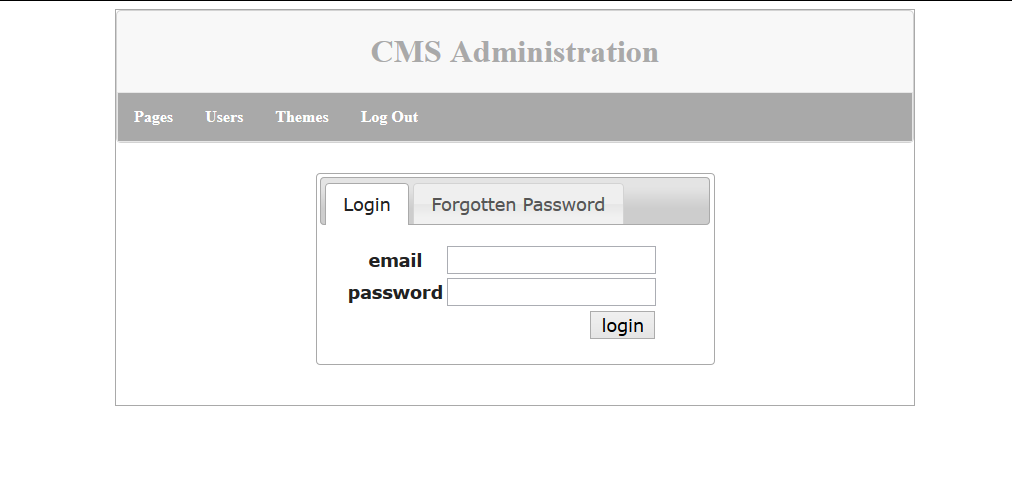
\includegraphics[width=\textwidth,height=\textheight,keepaspectratio]{pics/adminLoginPage.png}
    \caption{Landing Page}
\end{figure}



\subsubsection{Login}
Login page for the CMS is going to be designed in such a way that it will have a high Visibility. The user should know what to do as soon as he/she looks at the Login page.

\begin{figure}[H]
 \centering
    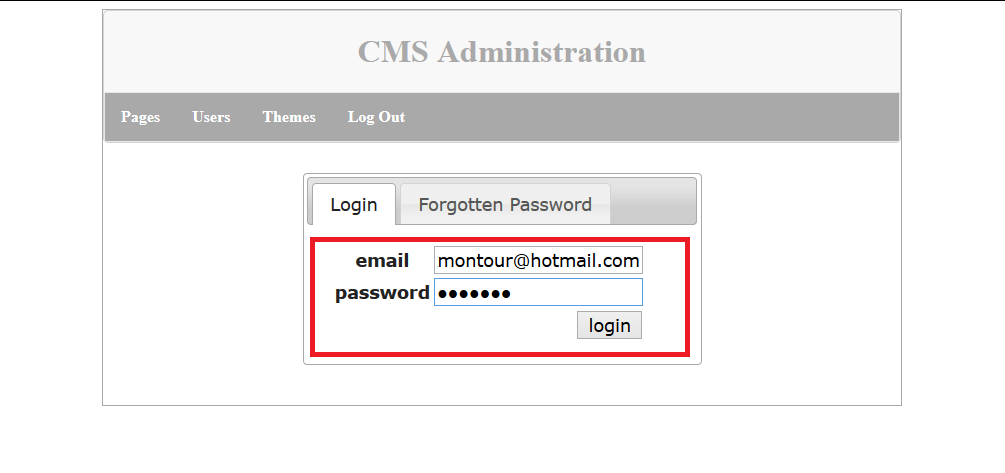
\includegraphics[width=\textwidth,height=\textheight,keepaspectratio]{pics/emailPassword.png}
    \caption{Login}
\end{figure}


\subsubsection{Navigation Menu}

\begin{itemize}
  \item All pages on the CMS have the same navigation layout for consistency. The rest of the space on each page is dedicated to the specific function of the page.
  \item Navigation menu structure is the same throughout the CMS to improve Learnability. The fonts, colors and layout of the navigation bar are also consistent.
\end{itemize}

\subsubsection{Create Basic User}
Navigating the CMS to create a basic user is very simple and easy to do since the navigation menu on each page has a menu item ''Users'' giving the task of creating a basic user a high Visibility.

\subsubsection{Edit User}
Similar to the create basic user task, Edit user task has a high visibility and therefore is easy to find for even the first time users since ''Users'' menu item is located in the navigation menu on every page.

\subsubsection{Delete User}
Similar to create basic user and edit user tasks, the delete user task has a high visibility since ''Users'' menu item is located in the navigation menu on every page. Thus making it easier for users to navigate the CMS if they want to delete a user.

\subsubsection{Logout}
The CMS allows the user to Logout at any moment of time and similar to Edit user task, Logout task has a high visibilty since ''Logout'' menu item is located in the navigation bar of every page, making logout easy and fast.

\subsubsection{Changing Theme}
The CMS allows for a users to change the theme of their site at any time. This task of changing the theme of the site has a high visibility since ''Themes'' menu item is located in the navigation bar on every page of the CMS.

\subsubsection{Edit / Add Page}
CMS allows users to edit/add pages easily through the "Pages" menu item which has a high visibility since it is located in the navigation bar of every page. Once the user clicks the "Pages" item the Page Management page comes up which has within it a "what you see is what you get" editor that allows the user to edit their pages with ease. This page editor has a high Affordance since the options within it are pretty much self explanatory and every button has a label or a symbol associated with it which makes it easy to understand.

\begin{figure}[H]
 \centering
    \includegraphics[width=\textwidth,height=\textheight,keepaspectratio]{pics/addPageThroughEditor.png}
    \caption{Login}
\end{figure}


\subsection{Feedback}
CMS provides users with efficient feedback so they know the actions they have conducted and the the actions they are about to conduct. Example of a feedback the CMS provides to the user is the feedback just before user deletes the account asking the user if they are sure that they want to delete the user account.

\begin{figure}[H]
 \centering
    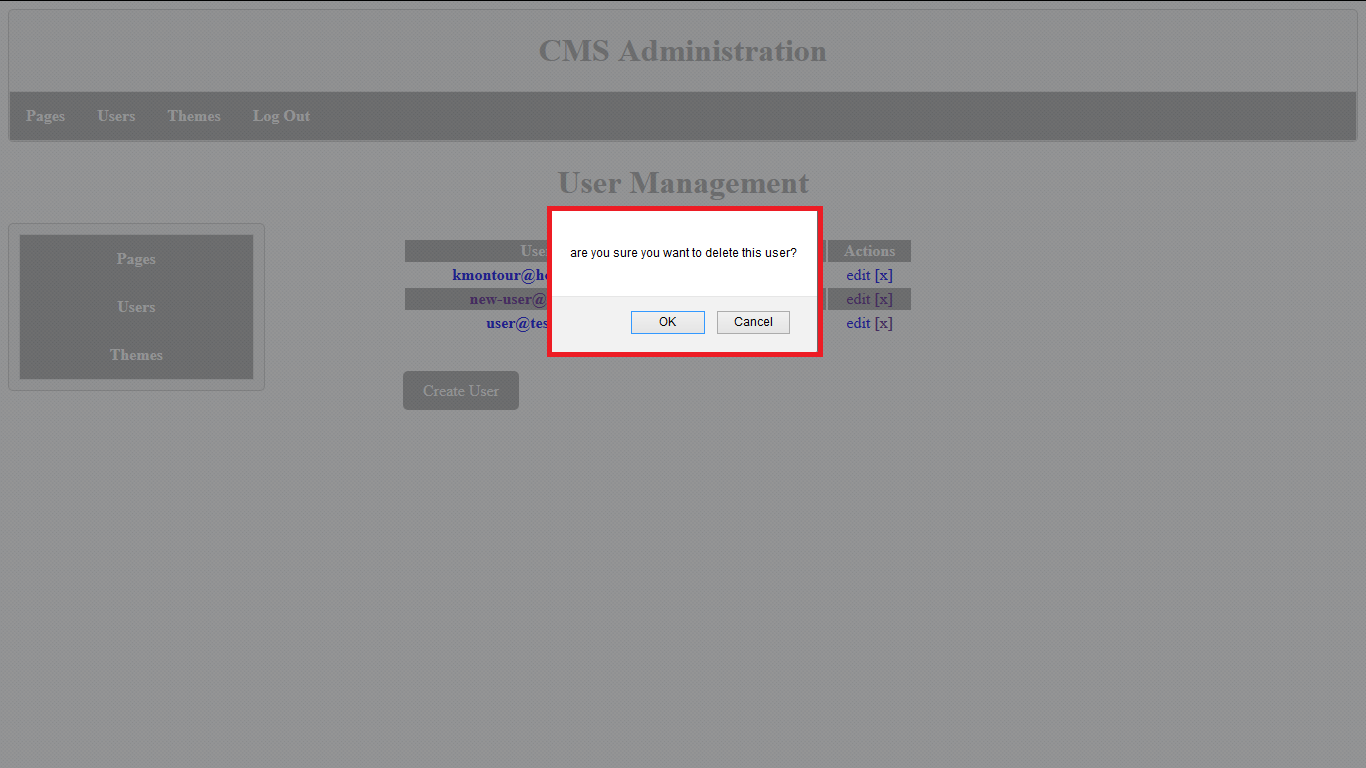
\includegraphics[width=\textwidth,height=\textheight,keepaspectratio]{pics/deleteUser_3.png}
    \caption{Deleting user feedback}
\end{figure}


\subsection{Consistency}
The CMS has a high consistency since page layout throughout the CMS is the same just the specific functionality for each page is different. Other than that fonts, colors and navigation menu is same on every page of the CMS.


\pagebreak


\begin{thebibliography}{9}
\bibitem{norman}
 Preece, J., Rogers, Y., Sharp, H. (2002)
\textit{ Interaction Design: Beyond Human-Computer Interaction}.
New York: Wiley, p.21.
\end{thebibliography}





\end{document}